\documentclass[11pt,a4paper]{article}

\usepackage[margin=2.5cm]{geometry}
\usepackage{amsmath, amssymb}
\usepackage{booktabs}
\usepackage{graphicx}
\usepackage[hidelinks]{hyperref}
\usepackage{cleveref}

\graphicspath{{../figures/}}

\title{Quantum Load Balancing for HPC Clusters:\\QAOA Simulated at Scale with GPUs}
% TODO(team): check names and add matriculation numbers if required.
\author{Xu Xia \and Denzel Elden Wijaya \and Keerthivasan \and Efe Kahraman}
\date{\normalsize SC4055 Group Project, November 2026}

\begin{document}
\maketitle

% Section 1 -- Introduction & Motivation (P2)
% Numbers in the findings paragraph come from results/E1_depth.csv and results/baselines_timing.csv.

\section{Introduction}
\label{sec:intro}

High-performance computing (HPC) clusters run many jobs at once, and a scheduler decides which job runs on which compute node.
A poor placement leaves one node overloaded while another sits idle, so every job on the busy node finishes late.
Placement also has to respect interactions between jobs: two memory-bound jobs placed on the same node compete for memory bandwidth and slow each other down, so schedulers let users declare \emph{anti-affinity} rules that keep such jobs apart.
Finding the best placement is a combinatorial problem.
Even the simplest version, splitting $n$ jobs between two nodes so that both finish at the same time, has $2^n$ possible placements and is NP-hard in general.

Quantum computers have been proposed as a new tool for problems of this kind.
The Quantum Approximate Optimization Algorithm (QAOA)~\cite{farhi2014} is one of the leading candidates for near-term quantum devices~\cite{preskill2018}.
It works in three steps.
The problem is first rewritten as an energy function, an Ising Hamiltonian, whose lowest-energy state is the best solution~\cite{lucas2014}.
A short, parameterised quantum circuit then prepares a quantum state that favours low-energy solutions.
Finally, a classical optimiser tunes the circuit's parameters.
Whether QAOA can ever beat the best classical methods is still an open question.

Large enough quantum hardware is not yet available to us, so we study QAOA by simulating it on classical computers.
Simulation is itself an HPC problem: storing the state of $n$ qubits takes $2^n$ complex numbers, so each extra qubit doubles both the memory and the work.
We use graphics processing units (GPUs) through NVIDIA's CUDA-Q platform~\cite{cudaq} to reach problem sizes that would be slow or impossible on a CPU.
HPC therefore appears twice in this project: as the application we schedule for, and as the tool that makes the study possible.

\subsection{Research questions}

We study a simplified version of the scheduling problem: place $n$ jobs on two nodes so that the workloads are as balanced as possible, while keeping conflicting jobs on different nodes.
We ask four questions.

\begin{enumerate}
  \item[\textbf{RQ1}] \textbf{Solution quality.} How close does QAOA get to the optimal schedule, and does it improve as the circuit gets deeper?
  \item[\textbf{RQ2}] \textbf{Classical comparison.} How does QAOA compare with classical methods such as simulated annealing and standard partitioning heuristics?
  \item[\textbf{RQ3}] \textbf{Noise robustness.} How much do realistic hardware errors degrade QAOA's performance?
  \item[\textbf{RQ4}] \textbf{HPC scalability.} How much faster are GPUs than CPUs for simulating these circuits, and how large a problem can we reach?
\end{enumerate}

\subsection{Scope}

This project does not aim to show that quantum computers beat classical ones.
At the problem sizes that can be simulated, classical methods win easily, and we show this directly.
Instead, we aim to provide three things:
\begin{enumerate}
  \item a correct formulation of a real-world scheduling problem for a quantum algorithm;
  \item a solid, reproducible implementation, in which every number and figure is produced by a script from a fixed random seed; and
  \item an honest analysis of where QAOA works, where it struggles, and why.
\end{enumerate}

\subsection{Summary of findings}
% All numbers are means over 10 instances per size, as in Section 7.

\paragraph{RQ1: quality.}
QAOA improves with every layer.
Its approximation ratio rises from $0.71$--$0.73$ for random guessing to $0.83$--$0.87$ with one layer and $0.93$--$0.97$ with six, for 8 to 20 jobs.
With six layers the probability that one sample is optimal falls from 24\,\% at $n = 8$ to 3.5\,\% at $n = 20$, but random guessing falls much faster, so QAOA's advantage over it grows from 19 to about $17{,}000$ times.
From three layers on, the best of 10{,}000 samples is an exact optimum on every instance.
Angles also transfer between problem sizes: starting from angles found at $n = 8$ matches INTERP's quality with 40\,\% of its circuit evaluations.

\paragraph{RQ2: classical comparison.}
QAOA's best sample matches the exact solver CP-SAT and simulated annealing, and beats greedy partitioning heuristics, which ignore conflicts.
But classical methods are far faster at these sizes: CP-SAT finds and proves the optimum for 28 jobs in about 5\,ms, while a single QAOA circuit evaluation at $n = 20$ already takes 30\,ms on a GPU, and optimisation needs hundreds of them.

\paragraph{RQ3: noise.}
A two-qubit error rate of 0.1\,\% costs little, but at 1\,\% extra layers stop helping after $p = 2$, and four layers do worse than one.
Noise therefore caps the useful circuit depth.

\paragraph{RQ4: HPC scalability.}
At $n = 20$ one circuit evaluation takes 76\,s on the CPU and 0.03\,s on an NVIDIA A40 GPU, about $2{,}500$ times faster, and the GPU reaches 30 qubits.
Reusing angles from $n = 20$ without any optimisation still gives an approximation ratio of $0.90$ at $n = 28$.
The GPU speeds up the simulation, but its cost still doubles with every qubit.

\subsection{Outline}

Section~\ref{sec:background} introduces Ising models, QAOA and GPU simulation.
Section~\ref{sec:formulation} turns the scheduling problem into a Hamiltonian.
Sections~\ref{sec:method} and~\ref{sec:implementation} describe the QAOA method and its CUDA-Q implementation, and Section~\ref{sec:setup} describes the experiments.
Section~\ref{sec:results} presents the results, Section~\ref{sec:discussion} discusses them and their limitations, and Section~\ref{sec:conclusion} concludes.

% Section 2 -- Background (P2)
% Needs: \usepackage{amsmath, amssymb, booktabs}

\section{Background}
\label{sec:background}

\paragraph{Ising models.}
Many combinatorial problems can be written as an Ising model: minimise $C(z) = c_0 + \sum_i h_i z_i + \sum_{i<j} J_{ij} z_i z_j$ over spins $z_i \in \{+1, -1\}$~\cite{lucas2014}.
Constraints are added as penalty terms.
Replacing each $z_i$ by the Pauli operator $Z_i$ gives a Hamiltonian $H_C$ that is diagonal in the computational basis, whose eigenvalue on $\lvert x \rangle$ is the cost of that assignment ($z_i = 1 - 2x_i$), so its ground state is the optimal solution.

\paragraph{QAOA.}
QAOA~\cite{farhi2014} starts from the uniform superposition $\lvert + \rangle^{\otimes n}$ and applies $p$ layers, each a cost layer $e^{-i\gamma H_C}$ followed by a mixer $e^{-i\beta H_M}$ with $H_M = \sum_i X_i$:
\begin{equation}
  \lvert \boldsymbol\gamma, \boldsymbol\beta \rangle
  = e^{-i\beta_p H_M} e^{-i\gamma_p H_C} \cdots e^{-i\beta_1 H_M} e^{-i\gamma_1 H_C} \lvert + \rangle^{\otimes n}.
\end{equation}
The cost layer gives each assignment a cost-dependent phase, and the mixer turns phase differences into amplitude differences, so with good angles low-cost assignments become more likely.
A classical optimiser tunes the $2p$ angles to minimise $\langle H_C \rangle$, and the final circuit is measured many times, each shot giving one candidate solution.
As $p \to \infty$ QAOA can imitate adiabatic evolution and reach the ground state~\cite{farhi2014}; at small $p$ it is approximate, and because the energy landscape has many local minima, the starting angles matter.
INTERP~\cite{zhou2020} starts depth $p + 1$ by interpolating the optimised angles of depth $p$.

\paragraph{GPU simulation.}
A statevector simulator stores all $2^n$ amplitudes (8\,GiB for 30 qubits in single precision, 16\,GiB in double), and every gate updates every amplitude: many simple, independent updates to one large array, which suits GPUs.
CUDA-Q~\cite{cudaq} runs the same circuit on CPU or GPU simulators; noise needs a density matrix with $4^n$ entries, which limits our noise study to small $n$.

% Section 3 -- Problem Formulation (P2)
% Needs: \usepackage{amsmath, amssymb, booktabs}
% Every number here comes from src/problem.py or results/lambda_sweep.csv.

\section{Problem Formulation}
\label{sec:formulation}

\paragraph{Scheduling model.}
We place $n$ jobs on two identical nodes, A and B, with $z_i = +1$ for node A and $-1$ for node B.
Job $i$ has a normalised runtime $w_i = \tilde w_i / \max_k \tilde w_k \in (0, 1]$, and a conflict graph $E$ lists pairs of jobs that should not share a node.
With total work $W$ and load difference $D = \sum_i w_i z_i$, the makespan is $(W + |D|)/2$, so minimising it is the same as minimising $D^2$.
Without conflicts this is number partitioning~\cite{lucas2014, karmarkar1982}.

\paragraph{Instances.}
Runtimes are heavy-tailed, like real HPC jobs: $\tilde w_i = \max(1, \operatorname{round}(e^{X_i}))$ with $X_i \sim \mathcal{N}(2, 1)$.
All conflicts can be satisfied only if $E$ is bipartite, so we \emph{plant} a hidden random split of the jobs into two halves and keep each pair across the split as a conflict with probability $0.2$, so every instance has at least one conflict-free schedule.
The runtimes are independent of the hidden split, so the solver must still trade balance against conflicts.

\paragraph{Cost function and Hamiltonian.}
The cost adds a penalty for conflicts to the balance term:
\begin{equation}
  C(z) = \Big( \sum_{i} w_i z_i \Big)^2 + \lambda \sum_{(i,j) \in E} z_i z_j
  = \sum_i w_i^2 + \sum_{i<j} J_{ij} z_i z_j,
  \qquad
  J_{ij} = 2 w_i w_j + \lambda \, \mathbb{1}[(i,j) \in E].
  \label{eq:ising}
\end{equation}
For a conflict edge, $z_i z_j = +1$ if both jobs share a node, so each violated conflict adds $2\lambda$ to the cost.
The balance term couples every pair of jobs, so the Ising graph is complete with $n(n-1)/2$ couplings.
Replacing $z_i$ by $Z_i$ gives the cost Hamiltonian
\begin{equation}
  H_C = \frac{1}{s} \Big( \sum_i w_i^2 \, I + \sum_{i<j} J_{ij}\, Z_i Z_j \Big),
  \label{eq:hamiltonian}
\end{equation}
whose eigenvalue on $\lvert x \rangle$ is $C(z)/s$.

\paragraph{Normalisation.}
\label{sec:normalisation}
We divide by $s = \max_{i<j} |J_{ij}|$ so that the largest coupling is exactly 1.
This does not change the optimum, but gives every instance the same scale for $\gamma$, so that the energy does not oscillate too fast in $\gamma$ for the optimiser and angles can be transferred between instances.
Energies are converted back with $C = s \langle H_C \rangle$ before any metric is computed.

\paragraph{Mirror symmetry.}
\label{sec:symmetry}
Swapping the two nodes, $z \mapsto -z$, never changes the cost, so every schedule has a mirror image with the same cost, and QAOA gives both exactly the same probability.
Integer runtimes often allow several balanced splits, and between 10\,\% and 45\,\% of our instances have more than two optimal bitstrings, so $P(\text{opt})$ counts \emph{all} of them.

\paragraph{Penalty weight.}
\label{sec:lambda}
A small $\lambda$ lets the optimum accept a conflict for better balance; a large $\lambda$ dominates $s$ and shrinks the balance couplings after scaling, which makes balance harder for QAOA to resolve.
We swept $\lambda \in \{0.1, 0.5, 1, 2, 5\}$ on 20 instances at each even $n$ from 6 to 24 and chose the smallest $\lambda$ whose optimum has zero violations on at least 90\,\% of instances at every size.
At $\lambda = 0.1$ this fraction drops to 50\,\% at $n = 24$, while $\lambda = 0.5$ reaches 90--100\,\% everywhere, so we use $\lambda = 0.5$.
We report violations as a separate metric for every method.

% Uncomment each line once its file exists.
% Section 4 -- Method (P1)
% Every setting here comes from src/qaoa.py, src/problem.py or experiments/E1_depth.py.

\section{Method}
\label{sec:method}

This section describes how we build, optimise and evaluate the QAOA circuit for the cost Hamiltonian $H_C$ of Eq.~\eqref{eq:hamiltonian}.
Section~\ref{sec:qaoa-background} introduced the algorithm; here we fix the choices that the results depend on.

\subsection{Circuit}
\label{sec:circuit}

The circuit uses one qubit per job, with qubit $i$ holding job $i$.
It starts with a Hadamard gate on every qubit to prepare $\lvert + \rangle^{\otimes n}$ and then applies $p$ layers.
In layer $\ell$ the cost unitary $e^{-i\gamma_\ell H_C}$ factorises exactly into one two-qubit term per coupling, because all terms of $H_C$ commute.
Each term is compiled as
\begin{equation}
  e^{-i \gamma J_{ij} Z_i Z_j} = \mathrm{CX}_{ij}\; R_Z^{(j)}(2\gamma J_{ij})\; \mathrm{CX}_{ij},
  \label{eq:zz-gate}
\end{equation}
and the mixer $e^{-i\beta_\ell \sum_i X_i}$ is one $R_X(2\beta_\ell)$ rotation on every qubit.
The constant term of $H_C$ is a global phase and is not applied.
A layer therefore contains $n(n-1)$ CX gates, $n(n-1)/2$ $R_Z$ gates and $n$ $R_X$ gates, so the gate count grows as $n^2$ per layer and linearly in $p$.

The $2p$ angles are stored as one vector $\boldsymbol\theta = (\gamma_1, \dots, \gamma_p, \beta_1, \dots, \beta_p)$.
Because $H_C$ is real, the angles $\boldsymbol\theta$ and $-\boldsymbol\theta$ give complex-conjugate states with identical measurement probabilities.
Before we compare or average angles across instances, we therefore flip the sign of any vector with $\gamma_1 < 0$, so that all of them lie on the $\gamma_1 \geq 0$ branch.

\subsection{Objective and optimiser}
\label{sec:optimiser}

The optimiser minimises the exact expectation $E(\boldsymbol\theta) = \langle \boldsymbol\theta \rvert H_C \lvert \boldsymbol\theta \rangle$, which the simulator computes directly from the statevector.
Using the exact value instead of a shot estimate removes sampling noise from the optimisation, so the results isolate the behaviour of QAOA itself; on hardware, $E$ would have to be estimated from measurements.
Because $H_C$ is scaled so that $\max |J_{ij}| = 1$ (Section~\ref{sec:normalisation}), the same angle scale applies to every instance.

We use COBYLA, a gradient-free trust-region method, as implemented in SciPy, with an initial step of $0.2$\,rad and a budget of 500 energy evaluations per optimisation.
Gradient-free methods are the usual choice for QAOA because each gradient would cost $4p$ additional circuit evaluations.
We record the number of evaluations each run uses, since this is the main driver of simulation time.

\subsection{Initial angles}
\label{sec:init}

The energy landscape has many local minima, so the starting point matters.
We use four strategies; E1 uses the first, and E2 compares all four.

\begin{description}
  \item[Ramp ($p = 1$ only in E1).]
  A linear ramp that imitates a discretised annealing schedule: $\gamma_\ell = 0.75\,t_\ell$ and $\beta_\ell = 0.75\,(1 - t_\ell)$ with $t_\ell = (\ell - \tfrac12)/p$.
  \item[INTERP.]
  The method of Zhou et al.~\cite{zhou2020}.
  The optimised angles at depth $p$ are linearly interpolated onto $p + 1$ points and used as the starting point at depth $p + 1$:
  \begin{equation}
    \gamma^{(p+1)}_{\ell} = \frac{\ell - 1}{p}\, \gamma^{(p)}_{\ell - 1} + \frac{p - \ell + 1}{p}\, \gamma^{(p)}_{\ell},
    \qquad \ell = 1, \dots, p + 1,
  \end{equation}
  with $\gamma^{(p)}_0 = \gamma^{(p)}_{p+1} = 0$, and the same rule for $\boldsymbol\beta$.
  Each instance is therefore optimised as a chain $p = 1, 2, \dots, 6$, and depth $p + 1$ starts from a state at least as good as the optimum at depth $p$.
  \item[Random.]
  $\gamma_\ell$ uniform in $[0, \pi]$ and $\beta_\ell$ uniform in $[0, \pi/2]$; we keep the best of five starts.
  \item[Transfer.]
  The element-wise median of the optimised (sign-canonicalised) angles over the ten $n = 8$ instances of E1, used either as a starting point or directly with no optimisation.
  Optimal QAOA angles are known to concentrate across instances of the same problem class, so angles found on small instances are often good on larger ones.
\end{description}

\subsection{Sampling and metrics}
\label{sec:metrics}

After optimisation the circuit is measured 10{,}000 times, and each bitstring is mapped to a schedule with $z_i = 1 - 2x_i$.
Every instance used in E1 and E2 has at most 20 jobs, so we compute its exact minimum $C_{\min}$, maximum $C_{\max}$ and the full set of optimal bitstrings by brute force over all $2^n$ schedules.
For $n > 24$ (E5) the minimum comes from CP-SAT and $C_{\max}$ from a closed form.
We report four metrics.

\begin{enumerate}
  \item \textbf{Approximation ratio} of the mean cost,
  \begin{equation}
    r = \frac{C_{\max} - \langle C \rangle}{C_{\max} - C_{\min}},
    \label{eq:approx-ratio}
  \end{equation}
  with $\langle C \rangle = s\,E(\boldsymbol\theta)$.
  It is 1 for a state concentrated on optimal schedules and 0 for the worst schedule.
  Because the cost is quadratic and its range is set by the worst schedule, the uniform superposition (random guessing) already scores $r \approx 0.71$--$0.73$ on our instances; this is the $p = 0$ reference.
  \item \textbf{Success probability} $P(\text{opt})$: the fraction of shots that return \emph{any} optimal bitstring (Section~\ref{sec:symmetry}).
  \item \textbf{Best sample}: the lowest-cost schedule among the 10{,}000 shots, reported as its own approximation ratio. This is the answer QAOA would return in practice, and it is the like-for-like comparison with classical solvers, which also return one schedule.
  \item \textbf{Violations and makespan} of the best sample, so that a schedule that trades a conflict for balance is always visible.
\end{enumerate}

Every run also records its wall time and number of energy evaluations.
Runs are identified by (experiment, instance, depth, initialisation, backend, precision, noise level, seed) and appended to a CSV file as soon as they finish, so an interrupted sweep resumes where it stopped and every figure is regenerated from these files by a single script.

\subsection{Validation}
\label{sec:validation}

Before running any experiment we checked the implementation against exact results with an automated test suite (40 tests).
With all angles at zero the circuit returns the uniform state and $\langle C \rangle = \sum_i w_i^2$; the energy from the simulator matches the probability-weighted cost computed from the exact statevector; the sampled mean cost matches the exact expectation within shot noise; every bitstring and its mirror image have the same probability (Section~\ref{sec:symmetry}); and the qubit ordering maps bit $i$ to job $i$.
As end-to-end checks, $p = 3$ on a 6-job instance reaches $r > 0.9$ and samples the optimum more than five times as often as random guessing, and optimised QAOA beats random sampling on both metrics at $n = 10$.
For the noise study (E6), every noiseless density-matrix result is checked against the statevector energy and the run stops if they disagree.

% Section 5 -- Implementation
% Every detail here comes from src/ and tests/.

\section{Implementation}
\label{sec:implementation}

The QAOA circuit is one CUDA-Q kernel that takes the couplings and angles as inputs, so the same code serves every instance and depth.
During optimisation, \texttt{observe} returns the exact energy without shots; once the angles are fixed, \texttt{sample} measures the final circuit.
We use the CPU target \texttt{qpp-cpu} (always fp64), the GPU target \texttt{nvidia} (fp32 by default, fp64 with one option) and \texttt{density-matrix-cpu} for noise.
Each run is saved to a CSV row with its seed, target and precision as soon as it ends, so an interrupted job restarts where it left off.

% Section 6 -- Experimental Setup
% Needs: \usepackage{amsmath, booktabs}
% Hardware and job details come from the Slurm job logs. Run counts come from results/.

\section{Experimental Setup}
\label{sec:setup}

All GPU runs and CPU timing runs ran as Slurm batch jobs on a shared university cluster.
Each node has two NVIDIA A40 GPUs with 48\,GB each, two 16-core CPUs and 192\,GB of main memory.
We used Python 3.11, CUDA-Q 0.16 and SciPy 1.17.
Each GPU job used one GPU, and every job had a 24-hour limit.
Table~\ref{tab:experiments} lists the settings of each experiment, all with $\lambda = 0.5$.
Above $n = 24$ we know only one optimal schedule and its mirror image, so $P(\text{opt})$ at those sizes may be slightly too low.

\begin{table}[h]
  \centering
  \caption{Settings of each experiment. Instances are counted per size. Sizes go up in steps of 2 except in E3, which uses every size. In E2, INTERP also runs depths 1, 3 and 5.}
  \label{tab:experiments}
  \begin{tabular}{@{}llllll@{}}
    \toprule
    Exp. & Purpose & Simulator & Sizes $n$ & Instances & Depth $p$ \\
    \midrule
    E1 & Depth sweep & CPU fp64 & 8--12 & 10 & 1--6 \\
       &             & GPU fp32 & 14--20 & 10 & 1--6 \\
    E2 & Starting angles & GPU fp32 & 10--16 & 10 & 2, 4, 6 \\
    E3 & Classical methods & none & 8--20 & 10 & none \\
       &                   & none & 21--28 & 1 & none \\
    E4 & Timing & CPU fp64 & 10--20 & 3 & 3 \\
       &        & GPU fp32 and fp64 & 10--30 & 3 & 3 \\
    E5 & Reused angles at large $n$ & GPU fp32 & 20--28 & 10 & 1--6 \\
    E6 & Gate noise & CPU density matrix & 6, 8 & 10 & 1--4 \\
    \bottomrule
  \end{tabular}
\end{table}

E4 changes only the target between runs.
Runs stop after different numbers of evaluations, so we compare the time per evaluation.
The CPU runs used 8 threads rather than the whole node.
Since qpp-cpu supports only fp64, the fair comparison is CPU fp64 against GPU fp64.
The nodes were shared, so timings reflect normal working conditions.
Two settings hit the 24-hour limit, which leaves one of three instances for GPU fp64 at $n = 30$ and two of three for the CPU at $n = 20$.

Because E1 mixes CPU fp64 and GPU fp32 results, we also ran $n = 12$ on the GPU.
The approximation ratio changed by less than 0.001 in 58 of 60 runs and the best sampled cost never changed, so fp32 does not affect our conclusions.

Precision also limits the largest problem a GPU can hold.
The simulator stores all $2^n$ amplitudes of the state, at 8 bytes each in fp32 and 16 bytes in fp64.
Each extra qubit doubles the memory, so a 48\,GB A40 holds at most 32 qubits in fp32 and 31 in fp64.

% Section 7 -- Results. One file per experiment so everyone can edit in parallel.
% Figures are paired onto four float pages: pipeline schematic + E1 (in 07_e1_depth); E2 + E6 (in 07_e2_init); E3; E4 + E5 (in 07_e4_backends).

\section{Results}
\label{sec:results}

Unless stated otherwise, every point is a mean over the same ten instances per size (seeds 0--9), and shaded bands show $\pm 1$ standard error.

% Section 7.1 -- E1: quality vs depth (P1)
% Numbers from results/E1_depth.csv and results/E2/E2_init.csv.

\subsection{E1: Solution quality and circuit depth}
\label{sec:e1}

E1 runs INTERP-initialised QAOA at $p = 1, \dots, 6$ on ten instances per size $n = 8, 10, \dots, 20$ (CPU for $n \leq 12$, A40 GPU above; at $n = 12$ both agree within $0.0005$ at five of six depths).

\begin{figure}[p]
  \centering
  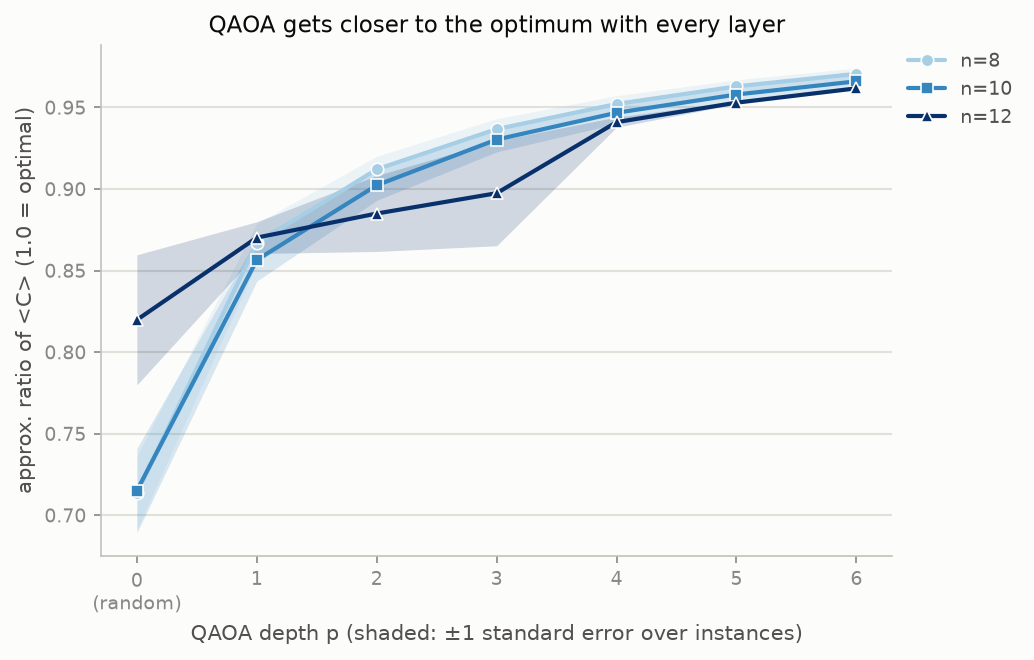
\includegraphics[width=0.8\linewidth]{E1_approx_ratio.png}\\[6pt]
  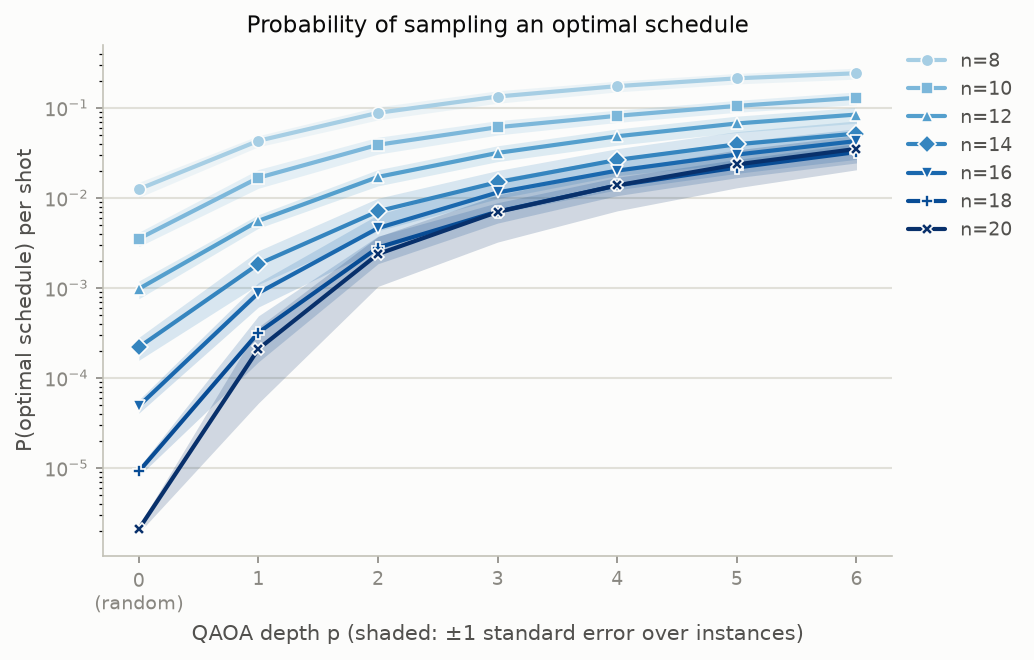
\includegraphics[width=0.8\linewidth]{E1_p_opt.png}
  \caption{E1. Top: approximation ratio of the mean cost against depth. Bottom: probability that one shot is optimal (log scale). $p = 0$ is random guessing.}
  \label{fig:e1}
\end{figure}

Quality improves with every layer (Fig.~\ref{fig:e1}, top): from $0.71$--$0.73$ for random guessing to $0.83$--$0.87$ at $p = 1$ and $0.93$--$0.97$ at $p = 6$.
No instance ever got worse with depth, but the gains shrink: at $n = 8$ layer 2 adds $0.045$ and layer 6 only $0.008$.
The dip at $n = 14$ and $16$ comes from two instances whose INTERP chain is stuck at $r \approx 0.73$ from $p = 1$ onwards; transferred angles reach $0.96$ and $0.92$ on them (E2), and without them both sizes average $0.95$.

$P(\text{opt})$ at $p = 6$ falls from $0.24$ at $n = 8$ to $0.035$ at $n = 20$ (Fig.~\ref{fig:e1}, bottom), but random guessing falls as $2^{-n}$, so QAOA's advantage grows from 19 to about $17{,}000$ times.
From $p = 3$ the best of 10{,}000 shots is an exact optimum on all 70 instances.
Single-precision GPU runs stop after about half as many COBYLA evaluations as CPU runs at the same quality, so we compare evaluation counts only within one precision.

% Section 7.2 -- E2: initialisation strategies (P2)
% Numbers from results/E2/E2_init.csv (p = 6, means over 10 instances per n).
% This file also holds the E6 figure, so E2 and E6 share one figure page.

\subsection{E2: Initialisation strategies}
\label{sec:e2}

E2 compares four starting points at $p = 6$ on the same ten instances per size $n = 10$--$16$: INTERP, the best of five random starts, and angles transferred from the $n = 8$ instances of E1, with and without optimisation.

\begin{figure}[p]
  \centering
  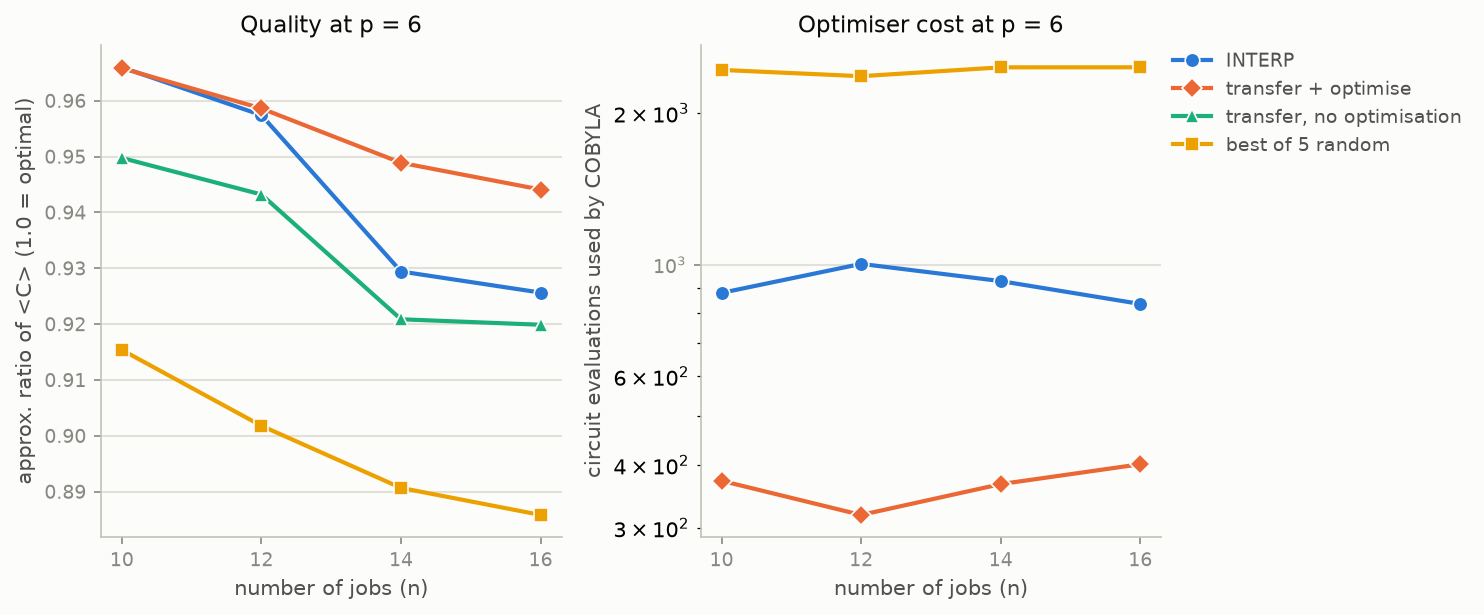
\includegraphics[width=\linewidth]{E2_init.png}
  \caption{E2 at $p = 6$. Left: approximation ratio of the mean cost. Right: circuit evaluations used by COBYLA (log scale); for INTERP this counts the whole chain $p = 1, \dots, 6$.}
  \label{fig:e2}
  \vspace{18pt}
  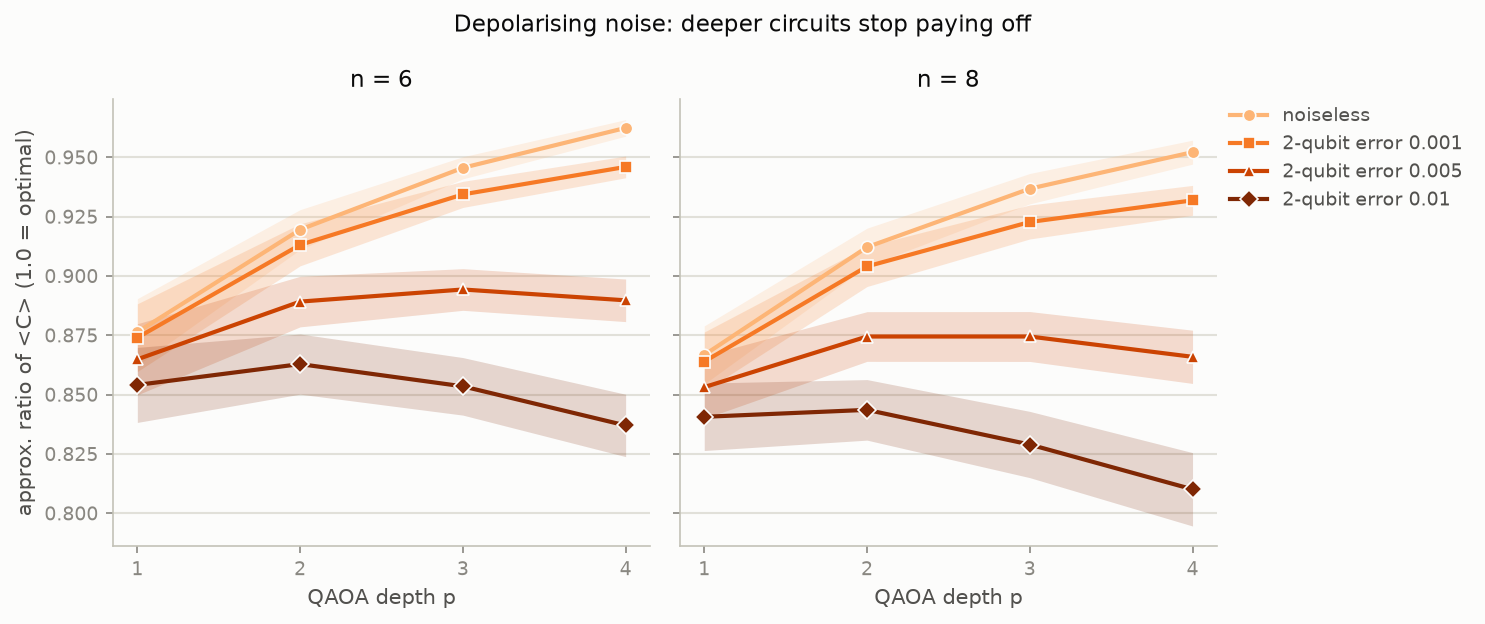
\includegraphics[width=\linewidth]{E6_noise.png}
  \caption{E6. Approximation ratio of the mean cost against depth for each two-qubit error rate, at $n = 6$ (left) and $n = 8$ (right).}
  \label{fig:e6}
\end{figure}

Transfer followed by optimisation gives the best quality at every size, with a mean ratio of $0.954$, against $0.945$ for INTERP, $0.933$ for transfer without optimisation and $0.898$ for random starts (Fig.~\ref{fig:e2}).
It is also cheap: about 360 evaluations, 40\,\% of INTERP's 910 over its full chain and 15\,\% of the 2{,}430 used by random starts.
The gap to INTERP comes from only two instances: the two on which INTERP is stuck in E1, where transfer reaches $0.961$ and $0.915$; without them both average $0.955$.
Even with no optimisation, transferred angles reach $0.933$, so good angles are similar across instances and sizes, which E5 exploits.

% Section 7.3 -- E3: classical baselines and the quantum comparison (P3)
% Numbers from results/baselines_timing.csv and results/E1_depth.csv (QAOA at p = 6).

\subsection{E3: Classical baselines and the quantum comparison}
\label{sec:e3}

E3 runs four classical methods on every instance: Karmarkar-Karp (KK) and greedy LPT, which balance load only and ignore conflicts by design, and simulated annealing (SA) and CP-SAT, which optimise the full cost in Section~\ref{sec:formulation}, conflicts included.
Sizes $n = 8, \dots, 20$ use the same ten instances as E1, so the classical and quantum results are directly comparable; $n = 21, \dots, 28$ use one instance each, since repeating the exact reference ten times over is the slow part, not the baselines themselves.
The reference optimum is brute force up to $n = 24$ and CP-SAT above it (Section~\ref{sec:setup}).

\begin{figure}[p]
  \centering
  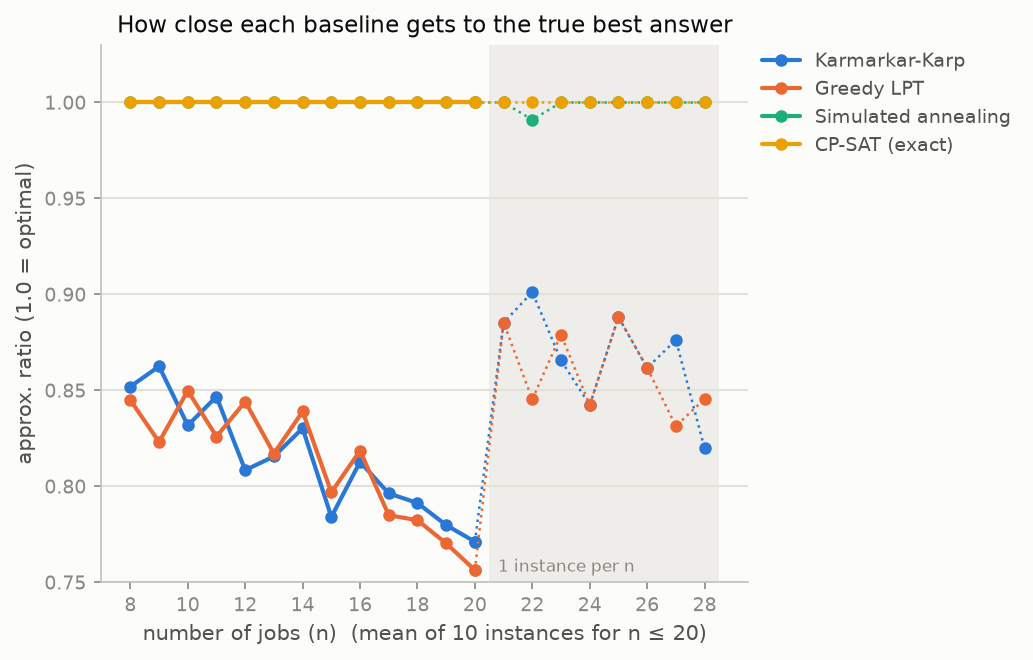
\includegraphics[width=0.8\linewidth]{baseline_approx_ratio.png}\\[6pt]
  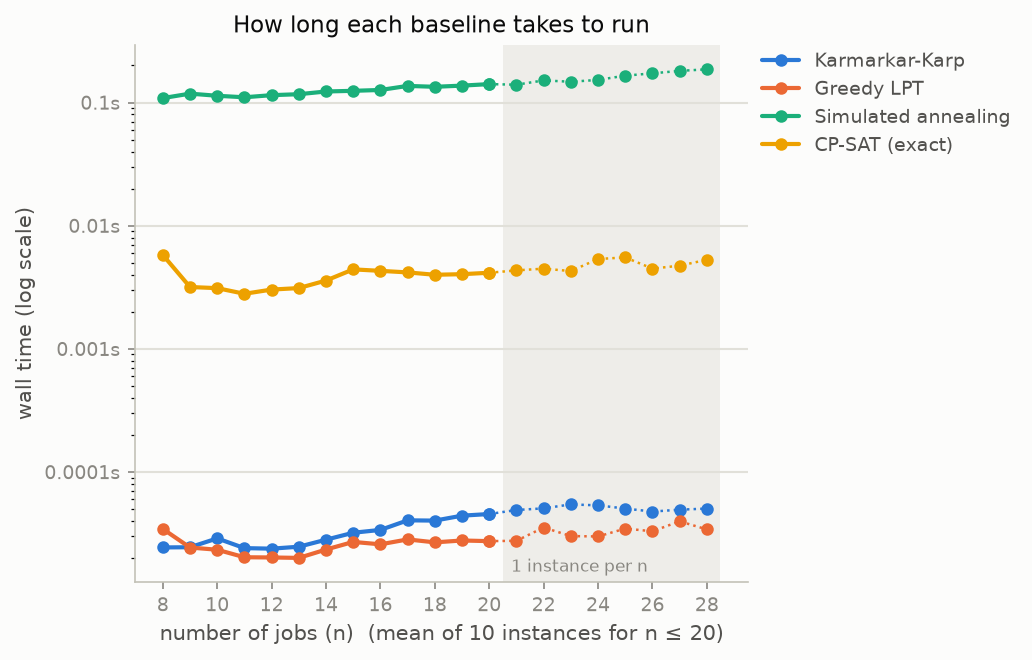
\includegraphics[width=0.8\linewidth]{baseline_wall_time.png}
  \caption{E3. Top: approximation ratio of each baseline's solution. Bottom: wall time (log scale). The shaded region past $n = 20$ has one instance per size rather than ten.}
  \label{fig:e3-baselines}
\end{figure}

KK and LPT land at $0.82$ and $0.81$ on average, with no clear trend in $n$ (Fig.~\ref{fig:e3-baselines}, top): since both ignore the conflict graph, their quality is set entirely by how evenly the balance term happens to split the planted weights, which does not get easier or harder as $n$ grows.
SA and CP-SAT are both effectively exact: CP-SAT finds the true optimum at every size by construction, and SA reaches a ratio of $1.0000$ at 136 of 138 runs, falling to $0.991$ at its worst.
This gap matters for conflicts specifically (Fig.~\ref{fig:e3-violations}): KK and LPT leave a mean of $5.06$ and $5.12$ violated edges per solution, while SA and CP-SAT leave $0.065$ and $0.058$, and find a fully conflict-free schedule on $93.5\,\%$ and $94.2\,\%$ of instances respectively -- consistent with $\lambda = 0.5$ being calibrated for roughly $90\,\%$ zero-violation optima (Section~\ref{sec:formulation}).

\begin{figure}[t]
  \centering
  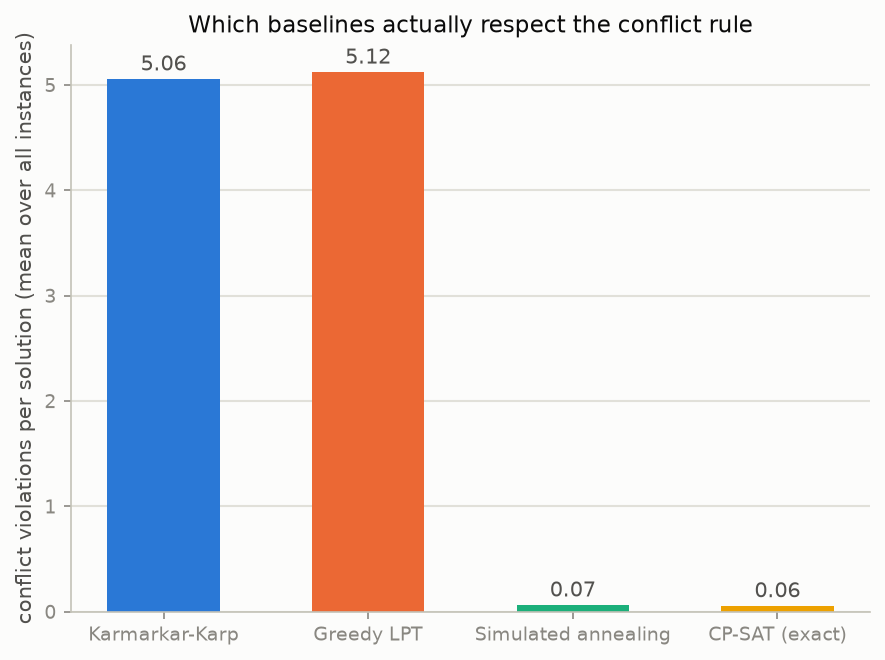
\includegraphics[width=0.6\linewidth]{baseline_violations.png}
  \caption{E3. Mean conflict violations per solution, averaged over all instances and sizes. KK and LPT never look at the conflict graph; SA and CP-SAT do.}
  \label{fig:e3-violations}
\end{figure}

Speed separates the two exact-ish methods sharply (Fig.~\ref{fig:e3-baselines}, bottom).
KK and LPT finish in tens of microseconds.
CP-SAT, despite being exact, is almost as fast: a mean of $3.9$\,ms and a worst case of $31$\,ms, including $5.3$\,ms to prove the optimum at $n = 28$.
SA is the slowest baseline at a mean of $126$\,ms, because it always runs its full $20{,}000$-iteration cooling schedule regardless of $n$, while CP-SAT's branch-and-cut exploits the structure of these instances directly.

\begin{figure}[t]
  \centering
  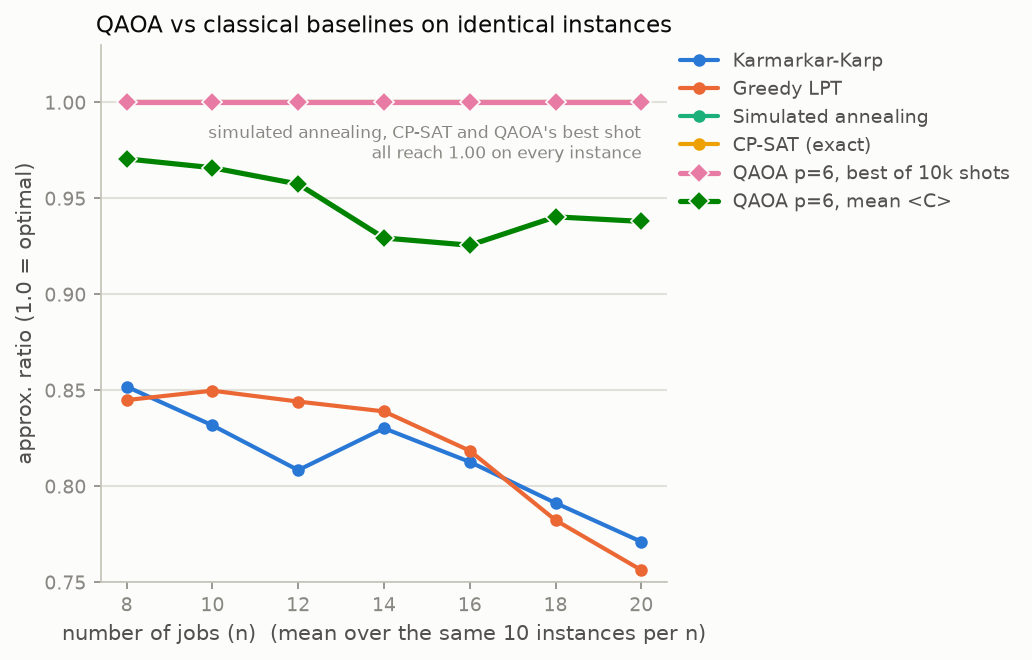
\includegraphics[width=0.8\linewidth]{qaoa_vs_baselines.png}
  \caption{QAOA's best depth ($p = 6$) against all four baselines, at the sizes where both have data ($n = 8$--$20$).}
  \label{fig:qaoa-vs-baselines}
\end{figure}

This answers RQ2 directly (Fig.~\ref{fig:qaoa-vs-baselines}).
QAOA at $p = 6$ beats both KK and LPT at every size tested, with approximation ratios of $0.93$--$0.97$ against $0.76$--$0.85$.
It never beats SA or CP-SAT, which reach $1.0000$ at every size by construction.
So QAOA is clearly doing more than naive load balancing, but at these sizes the gap to the strongest classical methods is not closed, and CP-SAT solves the whole problem, exactly, in milliseconds -- the scope set out in Section~\ref{sec:intro}: no quantum advantage here, by design, not by accident.

% Section 7.4 -- E4: CPU vs GPU vs fp64 (P3)
% Numbers from results/E4_cluster/*/E4_timing.csv.
% This file also holds the E5 figure, so E4 and E5 share one figure page.

\subsection{E4: Backend scaling (RQ4)}
\label{sec:e4}

E4 fixes the circuit at $p = 3$ and changes only the target.
Runs stop after different numbers of evaluations, so we compare time per evaluation.
Two settings hit the 24-hour limit, leaving one of three instances for GPU fp64 at $n = 30$ and two of three for the CPU at $n = 20$.

\begin{figure}[p]
  \centering
  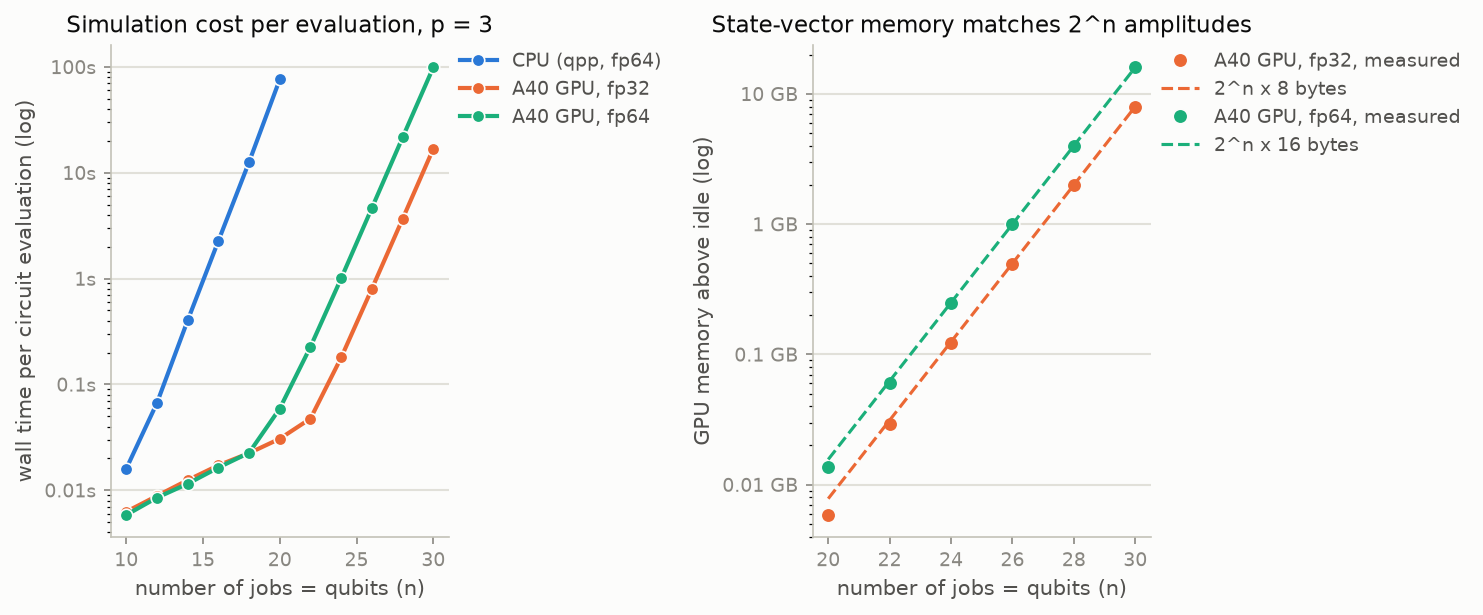
\includegraphics[width=\linewidth]{E4_timing.png}
  \caption{E4 at $p = 3$. Left: wall time per circuit evaluation (log scale). Right: GPU memory above an idle CUDA context against the $2^n$-amplitude prediction.}
  \label{fig:e4}
  \vspace{18pt}
  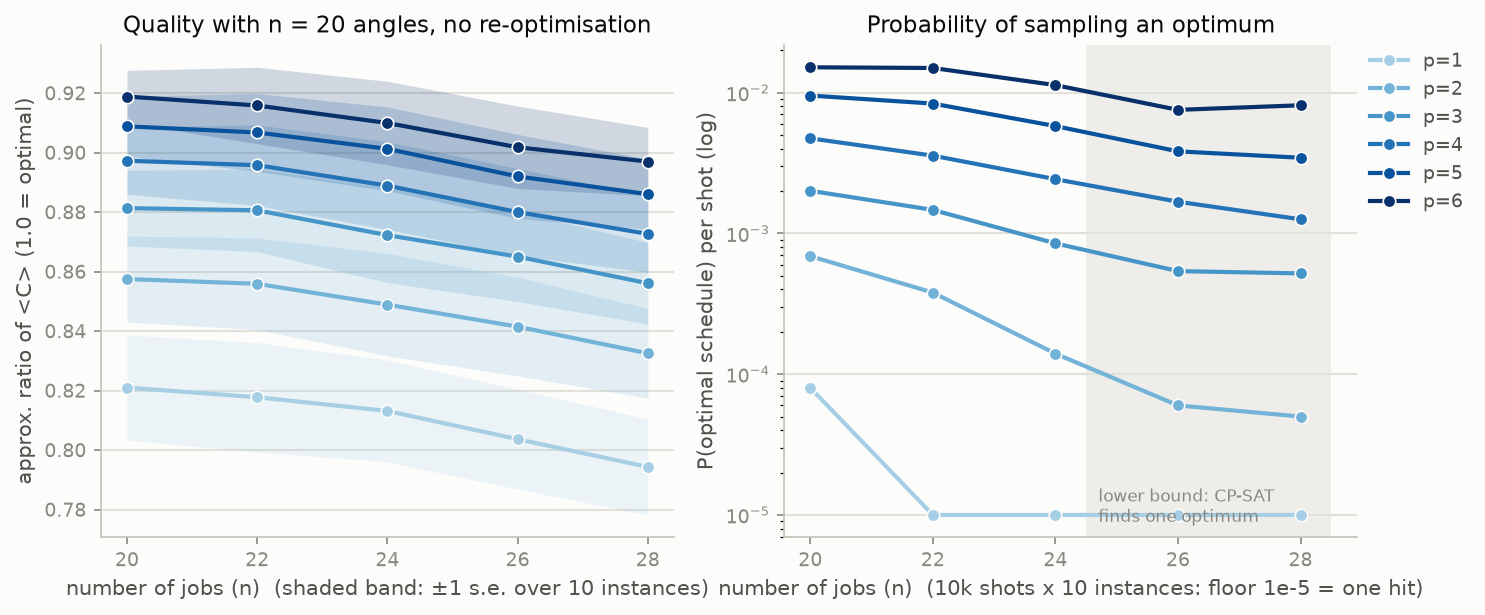
\includegraphics[width=\linewidth]{E5_largen.png}
  \caption{E5. Angles optimised at $n = 20$, reused without optimisation at $n = 20$--$28$. Left: approximation ratio by depth. Right: $P(\text{opt})$ (log scale), a lower bound above $n = 24$.}
  \label{fig:e5}
\end{figure}

At $n = 20$ the CPU takes $76$\,s and the GPU $31$\,ms, about $2{,}500$ times faster (Fig.~\ref{fig:e4}, left).
Each extra qubit doubles the amplitudes and the gate count also grows with $n$, so the CPU's cost grows five- to six-fold every two qubits, while the GPU stays nearly flat until about $n = 22$, where the work starts to fill it.
fp32 and fp64 cost about the same on the GPU up to $n = 18$, but fp64 is $1.9\times$ slower at $n = 20$ and $5.8$--$5.9\times$ slower from $n = 26$.
That is more than the $2\times$ of memory traffic alone, as the A40 has much lower fp64 throughput.
Measured GPU memory matches $2^n$ amplitudes at 8 or 16 bytes within 2\,\% from $n = 24$ (Fig.~\ref{fig:e4}, right), so one 48\,GB A40 holds at most 32 qubits in fp32 and 31 in fp64.

% Section 7.5 -- E5: large n with transferred angles (P3, angles from P1)
% Numbers from results/E5_cluster/E5_largen.csv and results/E1_depth.csv (n = 20, p = 6).
% The E5 figure lives in 07_e4_backends.tex so E4 and E5 share one figure page.

\subsection{E5: Large problems with transferred angles (RQ4)}
\label{sec:e5}

Optimising fresh angles at $n = 20$--$28$ is too slow, so E5 takes the median angles E1 optimised at $n = 20$ and samples with them at every size up to $n = 28$, with no optimisation (ten instances per size, 10{,}000 shots, GPU fp32).
Quality degrades gently: at $p = 6$ the ratio falls from $0.919$ at $n = 20$ to $0.897$ at $n = 28$ (Fig.~\ref{fig:e5}, left), although the search space grows 256-fold, and depth still helps throughout ($0.794$ at $p = 1$ for $n = 28$).
At $n = 20$, reusing angles instead of optimising each instance costs $0.02$ in ratio ($0.919$ against E1's $0.938$) and halves $P(\text{opt})$ ($0.015$ against $0.035$).
$P(\text{opt})$ at $p = 6$ falls to $0.008$ at $n = 28$ (Fig.~\ref{fig:e5}, right), and each run there takes about 12\,s.

% Section 7.6 -- E6: noise (P2)
% Numbers from results/E6/E6_noise.csv (means over 10 instances per n).

\subsection{E6: Robustness to noise}
\label{sec:e6}

E6 asks what happens when angles found on a perfect simulator are run on a noisy device.
We take the noiselessly optimised angles for ten instances at $n = 6$ and $8$ and depths $p = 1, \dots, 4$, and evaluate them without re-optimising under depolarising noise: each two-qubit (CX) gate fails with probability $p_{\text{err}} \in \{0, 0.001, 0.005, 0.01\}$, and each single-qubit gate with probability $p_{\text{err}}/10$.
We use CUDA-Q's density-matrix simulator, which is exact, so the results contain no shot noise; at $p_{\text{err}} = 0$ every run reproduces the noiseless energy.

\begin{figure}[t]
  \centering
  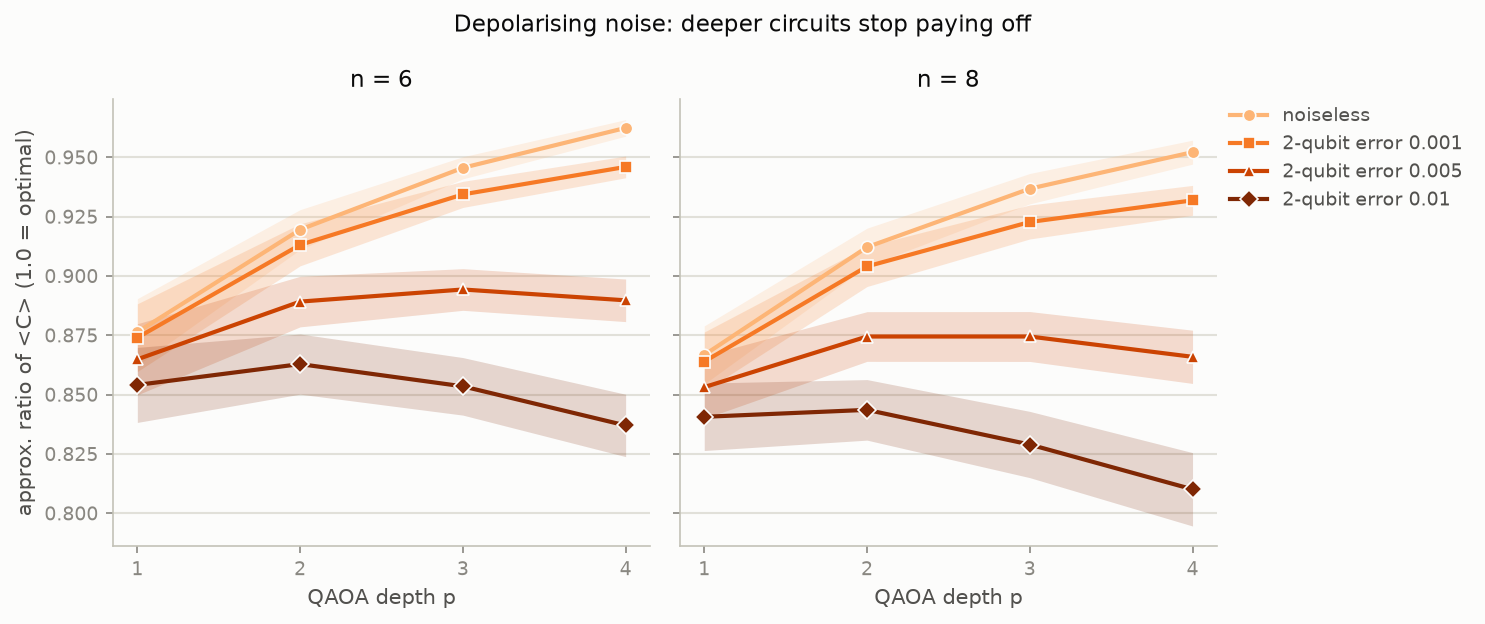
\includegraphics[width=\linewidth]{E6_noise.png}
  \caption{E6. Approximation ratio of the mean cost against depth for each two-qubit error rate, at $n = 6$ (left) and $n = 8$ (right). Bands show $\pm 1$ standard error.}
  \label{fig:e6}
\end{figure}

A small error rate costs little (Fig.~\ref{fig:e6}).
At $p_{\text{err}} = 0.001$ quality still improves with every layer and ends only $0.02$ below the noiseless value at $p = 4$ ($0.932$ against $0.952$ at $n = 8$).
At $0.005$ the improvement stops after two or three layers, at about $0.89$ for $n = 6$ and $0.874$ for $n = 8$.
At $0.01$ depth becomes harmful: at $n = 8$ the ratio falls from $0.841$ at $p = 1$ to $0.810$ at $p = 4$, and all ten instances end lower at $p = 4$ than at $p = 1$.
The success probability suffers more than the mean: at $n = 8$ and $p = 4$, $P(\text{opt})$ drops from $0.17$ without noise to $0.05$ at $p_{\text{err}} = 0.01$.

The cause is a trade-off between depth and gate count.
Each layer improves the ideal state, but also adds one $ZZ$ interaction, and so two CX gates, for every pair of jobs: 56 per layer at $n = 8$, and 224 at $p = 4$.
At $p_{\text{err}} = 0.01$, only $0.99^{224} \approx 10\,\%$ of runs pass through all of them without a two-qubit error.
Once the errors added by a layer outweigh its improvement, deeper circuits do worse, so the best depth depends on the hardware's error rate.
This noise model is simplified; Section~\ref{sec:discussion} discusses what it leaves out.


% Section 8 -- Discussion. GPU and precision paragraph from Efe (was 08_discussion_efe.tex).
% Numbers come from Section 7; nothing new is measured here.

\section{Discussion}
\label{sec:discussion}

\paragraph{Strengths and weaknesses of QAOA.}
Good angles are similar across instances and sizes, so transferred angles beat INTERP at lower cost (E2) and carry QAOA to $n = 28$ with no optimisation (E5), which matters most on real hardware, where every evaluation is slow and noisy.
QAOA's main cost is the optimisation loop: hundreds of evaluations, against milliseconds for CP-SAT (E3).
$P(\text{opt})$ also falls with $n$, so larger problems need more shots, and noise caps the useful depth at $p = 1$--$2$ at a 1\,\% error rate (E6).

\paragraph{GPU and precision.}
Our $2{,}500$-fold GPU speed-up at $n = 20$ is worth only about 11 extra qubits, because each qubit doubles the cost, and one 48\,GB A40 holds at most 32 qubits in fp32.
Single precision was the right choice on the A40.
From 24 qubits on it ran about six times faster than fp64, and in our check at $n = 12$ it never changed the best cost found.

\paragraph{Limitations.}
We schedule onto only two nodes; $k$ nodes would need several qubits per job and constraints to keep each job on exactly one node.
Above $n = 24$ we know only one optimum and its mirror, so $P(\text{opt})$ there is a lower bound.
Our noise model is depolarising only: it leaves out readout errors, decoherence and the SWAP gates that limited qubit connectivity would add, and we do not re-optimise angles under noise.
Finally, our timings are for simulation, not quantum hardware.

% Section 9 -- Conclusion.

\section{Conclusion}
\label{sec:conclusion}

We studied QAOA for two-node load balancing with anti-affinity constraints, simulated on GPUs with CUDA-Q.
QAOA improves with every layer, from $0.72$ for random guessing to $0.93$--$0.97$ at $p = 6$, and its best sample is optimal on every instance from $p = 3$ (RQ1).
It matches simulated annealing and CP-SAT on its best sample and beats greedy heuristics, but classical solvers are far faster at these sizes (RQ2).
At a two-qubit error rate of 1\,\%, depth beyond $p = 2$ makes results worse (RQ3).
An A40 GPU simulates these circuits about $2{,}500$ times faster than a CPU at $n = 20$ and reaches 30 qubits, and transferred angles carry QAOA to 28 jobs without optimisation (RQ4).
Next steps are scheduling onto more nodes, multi-GPU simulation beyond 30 qubits, and transferred angles on real hardware.


% Smaller, tighter references to stay within the 6-page text limit.
\let\oldthebibliography\thebibliography
\renewcommand{\thebibliography}[1]{\oldthebibliography{#1}\setlength{\itemsep}{0pt}}
\bibliographystyle{unsrt}
{\small\bibliography{references}}

\end{document}
